\chapter{Solar flare detection}

Before starting to write the main solar flare detection algorithm a first program was developed in which the location of the sun was known and we knew when the solar flare had taken place.

Try algorithm knowing the location of the source, sun. Show first distribution of VTEC thtough the day (vill), then for the specific moment in time


\section{Data}

To test this, the data used was that of the called "Hallowen Storm, in which 

\subsection{The Halloween Storm}

Halloween storm, poner ejemplos, citar al texto, porque esta tormenta otros papers de la storm tambien, decir que usaremos el momento exacto

\subsection{Formatting}
hablar de los datos, el formato, relevant to this algorithm: mappingion, d2li, etc

\subsection{AWK}

Usaremos awk, como va, muy breve



\section{VTEC distribution}

Fisrt we wanted to obtain VTEC distribution throughout the day, to see if any spikes appeared confirming that the moment we were going to study was correct.



\subsection{Computing the VTEC}

The Vtec...formulas...d2li/mappingio


\subsection{The solar flare}

Because the only operation that had to be performed was the previous division, a simple AWK script was used to filter out the two necessary fields from the data file (d2li and ) and print the resulting value and the time. 

\begin{lstlisting}[language=Awk, caption=process]
{
	/a/
	if ("vill" == $4) {
		d2li = $21;
		mappingFunc = $43;
		vtec = d2li/mappingFunc;
		print $3 " " vtec
	}
}
\end{lstlisting}

\begin{lstlisting}[language=Bash, caption=process]
#!/bin/bash
tiDataFile="../data/ti.2003.301.10h30m-11h30m.gz"
filename=vtecDistribution

zcat "$tiDataFile" | gawk -f previewVTECDistribution.awk > vtecValues
gnuplot -e "set terminal png; set output 'vtecDistribution.png'; set title 'VTEC Distribution'; set xlabel 'Time of the day (hours)'; set ylabel 'VTEC'; set grid; plot \"vtecValues\" using 1:2 with point"
rm vtecValues
\end{lstlisting}

The result can be seen in figure \ref{fig:vtecDistributionGeneral}

\begin{figure}[ht]
	\centering	
	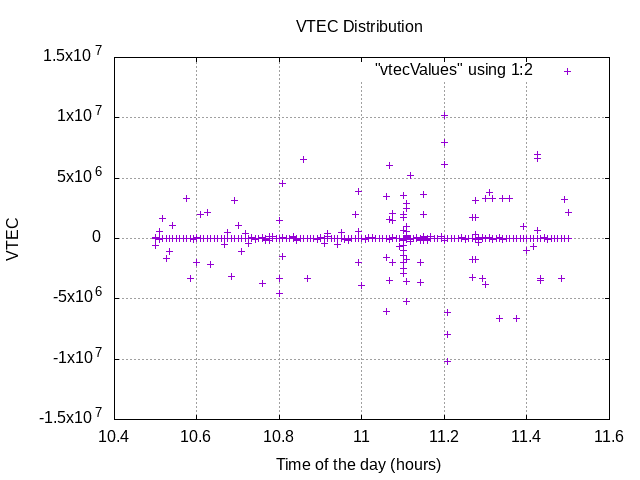
\includegraphics[width=0.6\linewidth]{images/ch4/vtecDistributionGeneral.png}
	\caption{VTEC distribution throughout the day for all IPPs}
	\label{fig:vtecDistributionGeneral}
\end{figure}

\begin{figure}[ht]
	\centering
	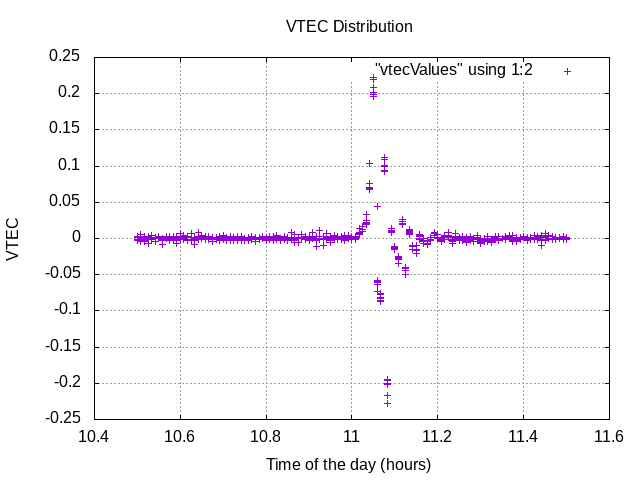
\includegraphics[width=0.6\linewidth]{images/ch4/vtecDistributionVill.png}
	\caption{VTEC distribution throughout the day for vVill}
	\label{fig:vtecDistributionVill}
\end{figure}


primer paso, ver datos de un IPP
Awk prepocesado de datos
fortran
gnu plot para empezar a ver

\section{Algorithm}

\subsection{VTEC value}

\subsection{Solar-zenith angle}









After that, talk about proposals for the main algorithm

explicar que vamos a hacer – IPPs, hill climbing y buscar si una vez en un pico, hay relacion lineal entre VTEC I coseno. En lugar de eso, subir mirando






\section{Pseudocode}

\begin{algorithm}
	\caption{My algorithm}\label{euclid}
	\begin{algorithmic}[1]
		\Procedure{MyProcedure}{}
		\State $\textit{stringlen} \gets \text{length of }\textit{string}$
		\State $i \gets \textit{patlen}$
		\BState \emph{top}:
		\If {$i > \textit{stringlen}$} \Return false
		\EndIf
		\State $j \gets \textit{patlen}$
		\BState \emph{loop}:
		\If {$\textit{string}(i) = \textit{path}(j)$}
		\State $j \gets j-1$.
		\State $i \gets i-1$.
		\State \textbf{goto} \emph{loop}.
		\State \textbf{close};
		\EndIf
		\State $i \gets i+\max(\textit{delta}_1(\textit{string}(i)),\textit{delta}_2(j))$.
		\State \textbf{goto} \emph{top}.
		\EndProcedure
	\end{algorithmic}
\end{algorithm}

\begin{lstlisting}[language=Python, caption=Python example]
import numpy as np

def incmatrix(genl1,genl2):
	m = len(genl1)
	n = len(genl2)
	M = None #to become the incidence matrix
	VT = np.zeros((n*m,1), int)  #dummy variable
	
	#compute the bitwise xor matrix
	M1 = bitxormatrix(genl1)
	M2 = np.triu(bitxormatrix(genl2),1) 
	
	for i in range(m-1):
	for j in range(i+1, m):
	[r,c] = np.where(M2 == M1[i,j])
	for k in range(len(r)):
	VT[(i)*n + r[k]] = 1;
	VT[(i)*n + c[k]] = 1;
	VT[(j)*n + r[k]] = 1;
	VT[(j)*n + c[k]] = 1;
	
	if M is None:
	M = np.copy(VT)
	else:
	M = np.concatenate((M, VT), 1)
	
	VT = np.zeros((n*m,1), int)
	
	return M
\end{lstlisting}

